% LTeX: language=en-GB
%Basics
\documentclass[a4paper, english]{article}
\usepackage[utf8]{inputenc}
\usepackage[T1]{fontenc}
\usepackage[bitstream-charter, cal=cmcal]{mathdesign}
\usepackage{babel}
\usepackage{csquotes}
\usepackage[moderate, mathspacing=normal]{savetrees}
%Author(s), Course variables
\newcommand{\lb}{\\}
\newcommand{\titl}{Verification of digital circuits using Java\xspace}
\newcommand{\auth}{Rasmus Wiuff\xspace}
\newcommand{\NO}{s163977\xspace}
\newcommand{\presub}{02125\xspace}
\newcommand{\aftersub}{Bachelor Project\xspace}
\newcommand{\datum}{\nth{12} of May 2025}
%Symbols and scientifics
\usepackage{bm}
\usepackage{physics}
\usepackage{mathtools}
\numberwithin{equation}{section}

% ------------------------------------------
%      For siunitx insert siux snippet      
% ------------------------------------------

%Appendix, TOC and Bibliography
\usepackage{appendix}
% \renewcommand\appendixtocname{Bilag}
\usepackage[nottoc]{tocbibind}
\setcounter{tocdepth}{2}
\usepackage{lastpage}

%Figures
\usepackage[svgnames]{xcolor} % Required to specify font color
\usepackage{float}
\usepackage{graphicx}
    \graphicspath{{C:/Users/rwiuf/Dropbox/LaTeXgraphics}}
\newcommand{\documentlogo}{DTU}
\usepackage{subcaption}
\usepackage[format=plain,
    labelfont={bf,it,footnotesize},
    textfont={it,footnotesize}]{caption}
\captionsetup{font={stretch=0.9}}
\usepackage[centering, rmargin=2.5cm, tmargin=2.5cm, lmargin=2.5cm, bmargin=3.5cm]{geometry}
\usepackage[final]{pdfpages}
\usepackage{multirow}
\usepackage{fontawesome}
\usepackage{xspace}
\usepackage{tikz}
\usetikzlibrary{positioning, automata}
\usepackage{dirtree}

% ------------------------------------------
% For semantic tableaux insert treex snippet
% ------------------------------------------

%Header footer
\usepackage{fancyhdr}
\pagestyle{fancy}
\lhead{\titl \lb \presub \aftersub}
\chead{\includegraphics[width=.05\textwidth]{\documentlogo}}
\rhead{\auth \lb \NO}
\cfoot{Page \thepage\, of\, \pageref*{LastPage}}
\renewcommand{\headrulewidth}{0.4pt}
\renewcommand{\footrulewidth}{0.4pt}
\setlength{\headheight}{36.75034pt}
%Text tools
\usepackage{listings}
\usepackage{parcolumns}
\usepackage[super]{nth}
\usepackage[normalem]{ulem}
\usepackage{import}
\usepackage{lipsum}
\usepackage{microtype}
\usepackage[pdfencoding=auto, psdextra]{hyperref}
\hypersetup{
    colorlinks   = true, %Colours links instead of ugly boxes
    urlcolor     = blue, %Colour for external hyperlinks
    linkcolor    = blue, %Colour of internal links
    citecolor   = red %Colour of citations
}
\usepackage[capitalise]{cleveref}
\usepackage{tabularray}
\UseTblrLibrary{booktabs}
\usepackage{todonotes}
\usepackage{biblatex}
\addbibresource{bibliography.bib}

\usepackage[newfloat]{minted}
\setminted{fontsize=\small,
           linenos=true}
\usemintedstyle{tango}
\SetupFloatingEnvironment{listing}{listname=Listings}
\captionsetup[listing]{position=top, skip=-1pt}
\usepackage{dirtree}

%Definitions and new commands
\newcommand{\degr}{^{\circ}}
\newcommand{\me}{\mathrm{e}}

\newcommand{\on}[1]{\operatorname{#1}}
\newcommand{\ddd}[0]{, \ldots, } % , ...,

% Logic.
\newcommand{\fall}[0]{~\forall}
\newcommand{\exst}[0]{~\exists}
\newcommand{\is}[0]{\mathrel{:}}
\newcommand{\from}[0]{\mathop{~:~}}

% Sets.
\newcommand{\nin}[0]{\not\in}
\newcommand{\with}[0]{\mathrel{|}}
\newcommand{\powerof}[1]{\mathcal{P}\left(#1\right)} % P(Set)
\newcommand{\power}[1]{2^#1} % 2^Set
\newcommand{\len}[1]{\ensuremath{|#1|}}
\newcommand{\eset}[0]{\emptyset}

% Numbers.
\newcommand{\N}[0]{\mathbb{N}}
\newcommand{\Z}[0]{\mathbb{Z}}
\newcommand{\Q}[0]{\mathbb{Q}}
\newcommand{\R}[0]{\mathbb{R}}

% Functions.
\newcommand{\cif}[0]{\text{, if }}
\newcommand{\els}[0]{\text{, otherwise}}

% Probability.
\newcommand{\probs}[1]{\operatorname{Pr}{\left[#1\right]}}
\newcommand{\expected}[1]{\mathrm{E}[#1]}
\newcommand{\given}[0]{\mathrel{|}}

% Complexity.
\renewcommand{\O}[0]{\ensuremath{\mathcal{O}}} % Big-O-Notation

% Bit macros
\newcommand{\bitzero}{\text{\textcolor{DTUred}{\fontfamily{fvm}\selectfont 0}}}
\newcommand{\bitone}{\text{\textcolor{DTUred}{\fontfamily{fvm}\selectfont 1}}}

%Title and sectioning
\def\Vhrulefill{\leavevmode\leaders\hrule height 0.7ex depth \dimexpr0.4pt-0.7ex\hfill\kern0pt}
\usepackage{titlesec}
\definecolor{DTUred}{cmyk}{0, .91, .72, .23}
\definecolor{FMNgrey}{cmyk}{.73,.43,.53,.38}
%Use letters insted of numbers in section numbering
% \renewcommand{\thesection}{\Alph{section}}
% \renewcommand{\thesubsection}{\Alph{subsection}}

% -------------------------------------------
% For pseudocode setup insert pseudox snippet
% -------------------------------------------

\usepackage{titling}

\begin{document}

\titleformat{\section}[block]
{\normalfont\Large\scshape\filright\color{DTUred}}{\fbox{\thesection}}{1em}{}

\titleformat{\subsection}
{\titlerule
    \vspace{.8ex}%
    \normalfont\scshape\color{FMNgrey}}
{\thesubsection.}{.5em}{}

\titleformat{\subsubsection}[wrap]
{\normalfont\fontseries{b}\selectfont\filright}
{\thesubsubsection.}{.5em}{}
\titlespacing{\subsubsection}
{12pc}{1.5ex plus .1ex minus .2ex}{1pc}

\makeatletter
\newcommand{\github}[1]{%
   \href{#1}{\color{DTUred}\faGithub}%
}
\makeatother

\title{\vspace{-5em}\hspace{-2em}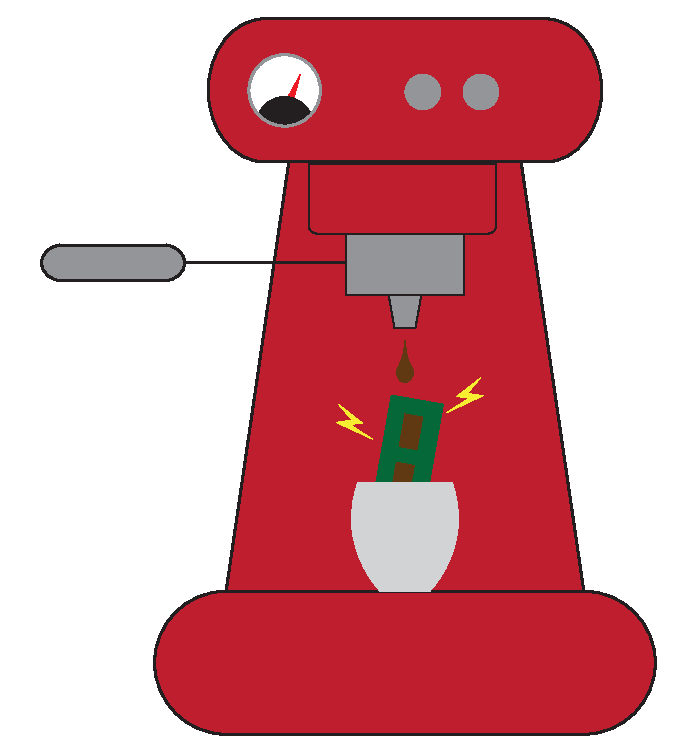
\includegraphics[width=.3\textwidth]{graphics/steelbrew.eps}\lb\vspace{.5em}\Huge\scshape\color{DTUred} \titl\lb\vspace{-4mm}\rule{4cm}{0.5mm}\lb\Large{\presub \aftersub}}
\date{\datum}
\preauthor{\begin{center}
        \large \lineskip 0.5em%
        \begin{tabular}[t]{ll}}
            \author{by & \\ \auth \textbf{\NO} & \href{mailto:s163977@dtu.dk}{s163977@dtu.dk} \\ \github{https://github.com/rwiuff/SteelBrew}\ \href{https://github.com/rwiuff/SteelBrew}{github.com/rwiuff/SteelBrew}\vspace{2.5em} \\ Supervisor & \\ Martin Schoeberl & \href{mailto:masca@dtu.dk}{masca@dtu.dk}}
            \postauthor{\end{tabular}\par\end{center}}

\maketitle

\begin{abstract}
    This project investigates the possibility of using a custom framework developed in Java to create testbenches and run these using Verilator, to verify digital circuit designs. The project implements core verification testing techniques, and successfully manage to evaluate these using multithreading. The project investigates the possibility of using Assertion Based Verification using Verilator, however does not succeed in doing so. The report finalise with showcasing the projects workflow for simple verification tests and discusses further possible improvements.
\end{abstract}

\pagenumbering{arabic}

\thispagestyle{empty}
\setcounter{page}{0}
\newpage
\tableofcontents
\addtocontents{toc}{~\hfill\textbf{Page}\par}
\setcounter{page}{1}
\newpage

% LTeX: language=en-GB
% !TeX root = ..\Thesis.tex
\section{Summary}\label{sec:01}
This section summarises the sections of the report.\newline
\cref{sec:02} surmises UVM and some chosen chip verification frameworks, pivoting towards the motivation for, and introduction of, this project.\newline
\cref{sec:03} breaks down the project into challenges and discusses solutions to these challenges.\newline
\cref{sec:04} goes through the design considerations along with diagrams outlining the projects intended structure.\newline
\cref{sec:05} describes the implementation and shows solutions of interest.\newline
\cref{sec:06} explains the testing used to verify the project.\newline
\cref{sec:07} summarises the project and discusses the results.\newline
% LTeX: language=en-GB
% !TeX root = ..\Thesis.tex
\section{Introduction}\label{sec:02}
\todo[inline]{Related works}
In the world of designing integrated systems on chips, it is crucial to describe these in some hardware description language in order to test designs before actual manufacturing. Part of testing these designs include writing tests in some framework supporting some abstraction and then simulate the chip using the applied framework, a process known as \emph{verification}. One verifies the \emph{Device Under Test} or DUT. One of the most common methodologies is \emph{Universal Verification Methodology}, or simply UVM.
\subsection{The UVM methodology}
Using UVM, one have to built testbench components. These include e.g. drivers for converting tests into proper DUT stimulus, monitors for reading the state of the DUT and scoreboards for comparing expected behaviour to actual behaviour, etc. UVM has the great benefit, that once these components have been defined, they can be reused within the scope of some system of designs. This means a high overhead, with high reusability.
\subsection{Current verification tools}
In today's landscape a myriad of verification tools exists. Projects like Chisel\footnote{On GitHub: \href{https://github.com/chipsalliance/chisel}{github.com/chipsalliance/chisel}}, and it's forked project SpinalHDL\footnote{On GitHub: \href{https://github.com/SpinalHDL/SpinalHDL}{github.com/SpinalHDL/SpinalHDL}} discards the traditional hardware description languages and testbenches altogether and implements their own, and pyuvm\footnote{On GitHub: \href{https://github.com/pyuvm/pyuvm}{github.com/pyuvm/pyuvm}} takes UVM into python using cocotb\footnote{cocotb on the web: \href{https://www.cocotb.org/}{www.cocotb.org/}} as a backend driver. These tools do however have some problems. Chisel and SpinalHDL requires developers to learn a new description language, which means the communities of developers are small, increasing slowly. pyuvm uses Python which itself is an interpreted language, meaning its runtime resource requirements do not scale well on large projects.
\subsection{The case against UVM and the mighty ABV}
Chip verification is inherently done by hardware designers and engineers and UVM is inherently created by and for hardware designers. When software engineers verify their software, they use unit tests and assertions along with formal proofs. In recent years these approaches have been adopted by hardware designers. \emph{Assertion Based Verification}, or ABV, along with formal verification is increasingly being applied to complex computing chip design verification and increases performance metrics over classic UVM\cite{reddy_formal_2024}. Key impacts from this paper is summarised on \cref{tbl:ABVOverUVM}.
\begin{table}[H]
    \centering
    \caption{Key impact of formal verification adoption over UVM\cite{reddy_formal_2024}}\label{tbl:ABVOverUVM}
    \begin{tabular}{l}
        \toprule
        Verification cycles reduced by 25-30\%             \\
        Pre-silicon bug detection rates improved by 20\%   \\
        Security vulnerability detection increased by 40\% \\
        \bottomrule
    \end{tabular}
\end{table}
\emph{SystemVerilog Assertions}, or SVA has been defined in IEEE 1800-2023\cite[Chapter 16]{noauthor_ieee_2024} meaning ABV is already a part of the SystemVerilog syntax.
\subsection{The goal of this project}
The goal of this project is a framework written in a strongly typed language, supporting SystemVerilog and core ideas from ABV, thus making it easy for designers to write their designs in SystemVerilog and use a well known language to implement assertion based tests.\newline Introducing \emph{SteelBrew}, the chip verification framework written in Java.
% LTeX: language=en-GB
% !TeX root = ..\Thesis.tex
\section{Related works}\label{sec:03}
In today's landscape a myriad of verification tools exists. Projects like Chisel\footnote{On GitHub: \href{https://github.com/chipsalliance/chisel}{github.com/chipsalliance/chisel}}, and it's forked project SpinalHDL\footnote{On GitHub: \href{https://github.com/SpinalHDL/SpinalHDL}{github.com/SpinalHDL/SpinalHDL}} discards the traditional hardware description languages and testbenches altogether and implements their own, and pyuvm\footnote{On GitHub: \href{https://github.com/pyuvm/pyuvm}{github.com/pyuvm/pyuvm}} takes UVM into python using cocotb\footnote{cocotb on the web: \href{https://www.cocotb.org/}{www.cocotb.org/}} as a backend driver. These tools do however have some problems. Chisel and SpinalHDL requires developers to learn a new description language, which means the communities of developers are small, increasing slowly. pyuvm uses Python which itself is an interpreted language, meaning its runtime resource requirements do not scale well on large projects.
As mentioned earlier ABV is increasingly becoming interesting as performance on verification of complex systems outperforms UVM\cite{reddy_formal_2024}
% LTeX: language=en-GB
% !TeX root = ..\Thesis.tex
\section{Problem specification and analysis}\label{sec:04}
As mentioned in \cref{sec:02} this project aims to implement a testing framework for SystemVerilog designs, using core ideas of Assertion Based Verification, written in Java. This poses the following challenges:
\begin{itemize}
    \item \textbf{Simulation driver:} The framework needs to communicate with some simulation driver.
    \item \textbf{Peek-poke-step:} Signal manipulation needs to be implemented to set up and carry out assertion of behaviour.
    \item \textbf{Assertion-logic: } ABV logic has to be implemented in the framework.
    \item \textbf{Test translation:} The framework has to translate test logic from Java to SystemVerilog and create a testbench for test simulation.
    \item \textbf{Coroutines/concurrency:} As assertions can be time-invariant, it makes sense to implement concurrency or coroutines to efficiently execute the simulation.
\end{itemize}
\subsection{Simulation driver}
Driving the simulations is not part of the scope of this project. Instead, the simulations are run by a third-party tool using Java to invoke the tool and listen for the results. Verilator\footnote{Verilator on the web: \href{https://www.veripool.org/verilator/}{veripool.org/verilator}} is a fast and community-driven simulator for SystemVerilog, which supports SVA directives. Through testbenches it is possible to set up and test DUT's fairly easily.
\subsection{Peek-poke-step}
Using the Java BigInt class, some logic for manipulating bits needs to be implemented in order to set up tests. BigInt enables describing integers in other bases, as is common in hardware design or low-level programming.
\subsection{Assertion-logic}
There are some assertion directives of interest:
\begin{enumerate}
    \item Assert which raises an exception if some property does not hold.
    \item Cover which monitors the coverage of some property.
\end{enumerate}
These are the minimum that should be implemented. Some object for a test should be created and react if the driver raises an exception pertaining to the used directive.
The logic in the framework needs to adhere to the logic stated in the SVA documentation.
\subsection{Test translation}
Manipulation and assertions has to be properly translated into a testbench that, when run, carries out the verification. This should be done in a manner that translates the test logic into a series of strings that are placed correctly within a testbench.
\subsection{Coroutines/concurrency}
To optimise runtime, it is desirable to run tests concurrently. For this purpose there are two options:
\begin{enumerate}
    \item Java Runnable
    \item Coroutines
\end{enumerate}
\subsubsection{Java Runnable}
The Java Runnable interface\footnote{Documentation on Oracle: \href{https://docs.oracle.com/javase/8/docs/api/java/lang/Runnable.html}{docs.oracle.com/javase/8/docs/api/java/lang/Runnable.html}} enables thread creation and joining. Benefits include the native support for Java and the documentation and community surrounding developing with Runnable. The main disadvantage is that threads rely on the operating system's scheduler, thus removing some degree of control during execution, and in the worst case, if not run in an elevated mode, threads might not get priority to run.
\subsubsection{Coroutines}
Coroutines are described as ``light threads'' and enables a thread to control its own behaviour. This means threads can execute with a high degree of control. Disadvantages is that Java does not natively support coroutines. Solutions include hacking the JVM or using third party projects to execute coroutines. One such example is Javaflow\footnote{Javaflow on Apache: \href{https://commons.apache.org/sandbox/commons-javaflow/}{commons.apache.org/sandbox/commons-javaflow/}} from Apache Commons or an interesting project called ``Coroutines''\footnote{Coroutines on GitHub: \href{https://github.com/offbynull/coroutines}{github.com/offbynull/coroutines}} inspired by Javaflow.
\subsection{Goals and success criteria}
The discussed challenges and their solutions are listed on \cref{tbl:criteria}.
\begin{table}[H]
    \centering
    \caption{The projects challenges and success criteria}\label{tbl:criteria}
    \begin{tabular}{lll}
        \toprule
        \# & Challenge              & Success Criteria                                                            \\
        \midrule
        1  & Simulation driver      & Logic that launches Verilator and handles communication with the processes. \\
        2  & Peek-poke-step         & Logic that, using BigInt, manipulates wires and ports in the tests.         \\
        3  & Assertion-logic        & Logic that sets up assertion directives supported by the driver             \\
           &                        & and SVA to support ABV.                                                     \\
        4  & Test-translation       & Logic that translates the written test into a testbench that when executed, \\
           &                        & ensures the tests are carried out correctly.                                \\
        5  & Coroutines/concurrency & Implementation of concurrent execution of the simulations.                  \\
        \bottomrule
    \end{tabular}
\end{table}
SteelBrew will be developed in an Agile way, based on use-cases. This ensures that a viable product is ready after dealing with challenge 1, 2 and 4 as these deals with setting up basic test functionality. Afterwards assertion logic, concluding with coroutines.
% LTeX: language=en-GB
% !TeX root = ..\Thesis.tex
\section{Design}\label{sec:05}
The design of SteelBrew will take an Agile approach to get going with some framework for writing and running simple tests on devices written in SystemVerilog, using Java.
\subsection{Use cases}
Using SteelBrew should be as simple as possible. \cref{fig:usecases} shows an overview of the use cases for a developer.
\begin{figure}
    \centering
    \caption{Use case diagram for SteelBrew}\label{fig:usecases}
    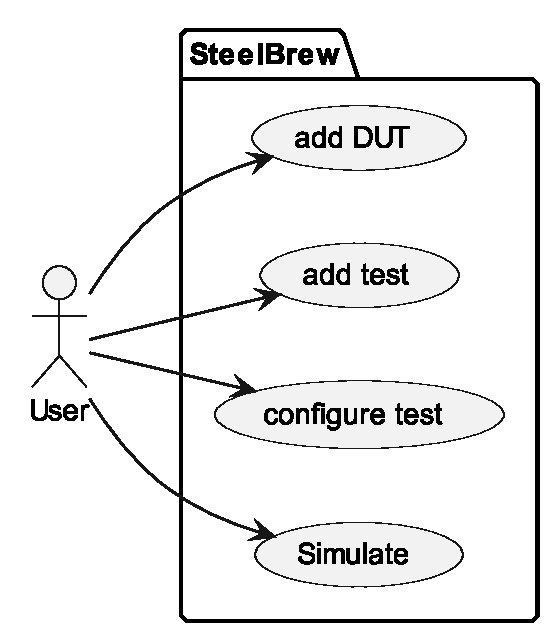
\includegraphics[width=.3\textwidth]{out/plantuml/usecase/usecase.eps}
\end{figure}
This is a simplification. As mentioned the framework is executed in Java, so to get started the user would start by creating a java project and importing SteelBrew. Hereafter the DUT is added and tests are defined and configured. A command should then execute the test and start the simulation.
\subsubsection{Adding the device under test}
With the device design in the root folder, adding it to the framework should be as easy as adding the device to some object that handles device configuration. The underlying logic should take care of the rest.
\subsubsection{Adding tests}
Since the tests are linked to some device, it is preferred that the same underlying logic ties tests and devices.
\subsubsection{Configure tests}
This is the bulk of the interaction for the user. With some object carrying the tests and device, the user should be able to easily add new tests or assertions with some easy to use method calls. The underlying logic should resolve conflicts and handle test creation without the user getting much involved.
\subsubsection{Simulate}
Since the simulations are carried out by a third-party program, all handling between SteelBrew and said program, should be handled by yet another class, separate from the test-driven class. This ensures good separation of responsibility in the project.
\subsection{Separation of responsibility}
The project is considered two-fold:
\begin{enumerate}
    \item Handling DUT's and tests
    \item Handling concurrency and third-party software
\end{enumerate}
For this reason the program has to contain two main components. The \emph{Brewer} and the \emph{Forge}.
A third class is introduced as the entry-point for the program, and will be accessible to all other classes. This class is simply \emph{SteelBrew}.
Expanding on \cref{fig:usecases}, the use case diagram is expanded as seen on \cref{fig:usecases2}.
\begin{figure}
    \centering
    \caption{The expanded use case diagram for SteelBrew}\label{fig:usecases2}
    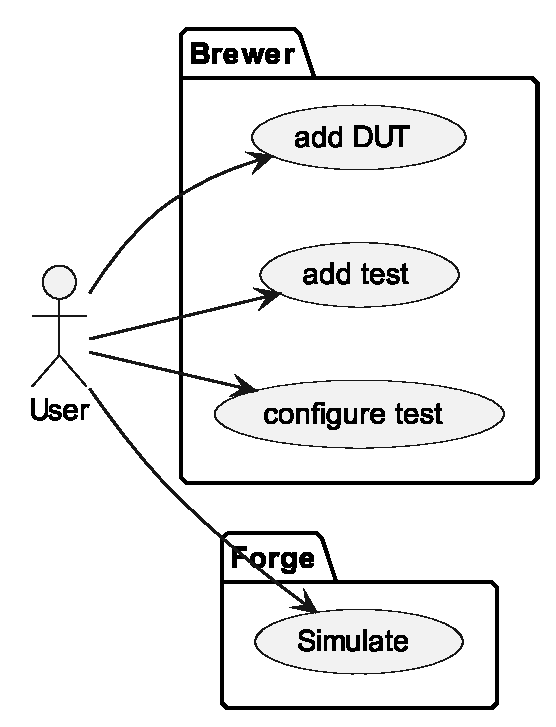
\includegraphics[width=.3\textwidth]{out/plantuml/usecase2/usecase2.eps}
\end{figure}
\subsection{The Brewer}
The Brewer is the primary interface. There are several ways of going about this object handling multiple DUT's and tests. One aspect could be to hold Lists or Maps of the tests and devices, and then use methods to get these, and couple them accordingly. This has the advantage that from a schematic point of view it simplifies the program. However, once tests are applied to different devices, all contained within the same object, one has to keep track of internal links. The first major decision in the design phase was as such:
\begin{enumerate}
    \item Give a Brewer to each DUT
    \item Assign tests to each Brewer
\end{enumerate}
This means more objects are created, but the Brewer object itself has a lot less responsibility in terms of tracking the internal links.\newline
A sequence diagram on \cref{fig:seqBrew} shows this initial idea.
\begin{figure}
    \centering
    \caption{Sequence diagram showing the idea behind the Brewer}\label{fig:seqBrew}
    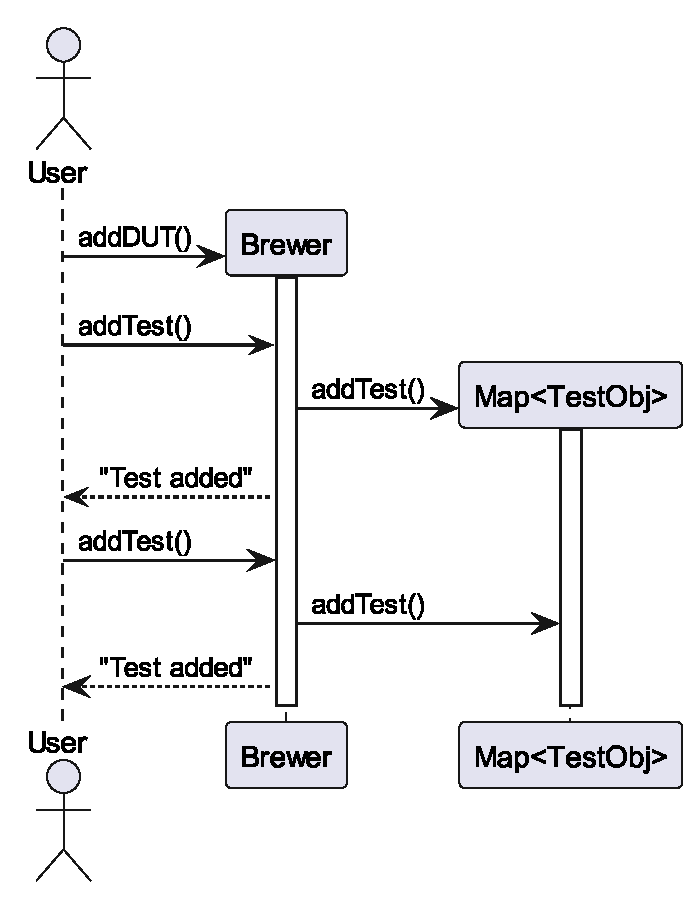
\includegraphics[width=.5\textwidth]{out/plantuml/Brewer/brewer.eps}
\end{figure}
\subsection{The Forge}
The Brewers complement, the Forge handles another job, entirely. This class has to handle the responsibility of taking the tests from the Brewers and hand them down to the third-party tool. This prompts some considerations, namely how to launch other programs with very specific parameters and how to communicate with these programs.
\subsubsection{Verilator and the Forge}
The third-party software chosen is Verilator. It is open-source and very quick at executing simulations. Verilator works like this:
\begin{enumerate}
    \item The user prepares testbenches describing the testing environment and the tests
    \item Verilator takes the testbench and some DUT as input and makes the files for compiling a C++ program
    \item Compiling and running the program executes the tests and outputs a waveform-file, which can be inspected by e.g. GTKWave.\footnote{GTKWave on the web: \href{https://gtkwave.sourceforge.net/}{gtkwave.sourceforge.net}}
\end{enumerate}

This puts constrains on the design of the program. The Forge needs to call Verilator multiple times and then needs to run the compiled program. To ease this, the program creates a Makefile and executes through this. Simple redirects of stdout means that the Forge can collect the output from Verilator and the simulation.
\subsubsection{Concurrency}
Up until now the main idea was to take a Brewer pointing to a DUT, add some tests and then hand it off to the Forge for Verilating, compiling and running the simulation. This poses one issue: This way of evaluating the program means that tests can only be parallised in terms of Verilator's internal multithreading, and then one DUT with all its test per thread. Verilator's internal multithreading is outside the scope of this project, so the only option is to get creative with the way tests are run. Normally when using Verilator, one testbench with all testing is run per DUT. The design choice here was to split up the tests, such that each test, or set of tests, gets its own testbench and its own compiled program. This way tests can be carried out in parallel by launching each workflow on different threads.
\subsubsection{Coroutines}
It was of great interest to involve coroutines in the project. Java does not support coroutines natively, so workarounds were investigated. To this end, it turns out most coroutine frameworks and plugins are 6+ years old. They do not support newer Java versions, and thus not newer Java functionality. The design choice here was to use threads to execute tests.
\subsection{Testbench}
The workflow of Verilator and the design choice of splitting up tests into separate executables meant that the definition of tests were somewhat straightforward. The Brewer would have Testbench objects. Whenever tests are defined they are added to this object, and just before simulation, testbench files are created based on the content of the object. The testbenches have to have unique names, otherwise the Verilator executable and GNU Make will be unable to execute the correct benches.
\subsection{Batch}
While the Testbench class is able to contain all tests put in, it is basically a collection of strings. Furthermore, it is often desirable to control the sequence in which tests are executed, as the result from one test might affect the other. Or if one has to test what happens when manipulating signals inside the DUT. A new class is introduced to handle a sequence of tests, along with logic transforming simple methods into cumbersome strings for the testbench. The Batch class keeps a record of signals and tests involved in some scenario and when ready, creates a testbench with these tests executed as they are added by the user.
The functionalities here starts with:
\begin{itemize}
    \item \textbf{Peek} Read signal
    \item \textbf{Poke} Change signal
    \item \textbf{Step} Increment DUT clock
\end{itemize}
\subsection{Assertions}
The last leg of the project is assertion support. Assertions is a formal way of ensuring certain properties of a design, either in the scope of its entire execution or in certain scenarios. SystemVerilog has long supported assertions, however Verilator has limited support for assertions. For this reason some core functionality is designed and implemented, namely relations between signals in the DUT, using logic and relational operators.
\subsection{Design overview}
The workflow is illustrated by the sequence diagram shown on \cref{fig:usecasesfinal}.
\begin{figure}
    \centering
    \caption{Final workflow example as a sequence diagram}\label{fig:usecasesfinal}
    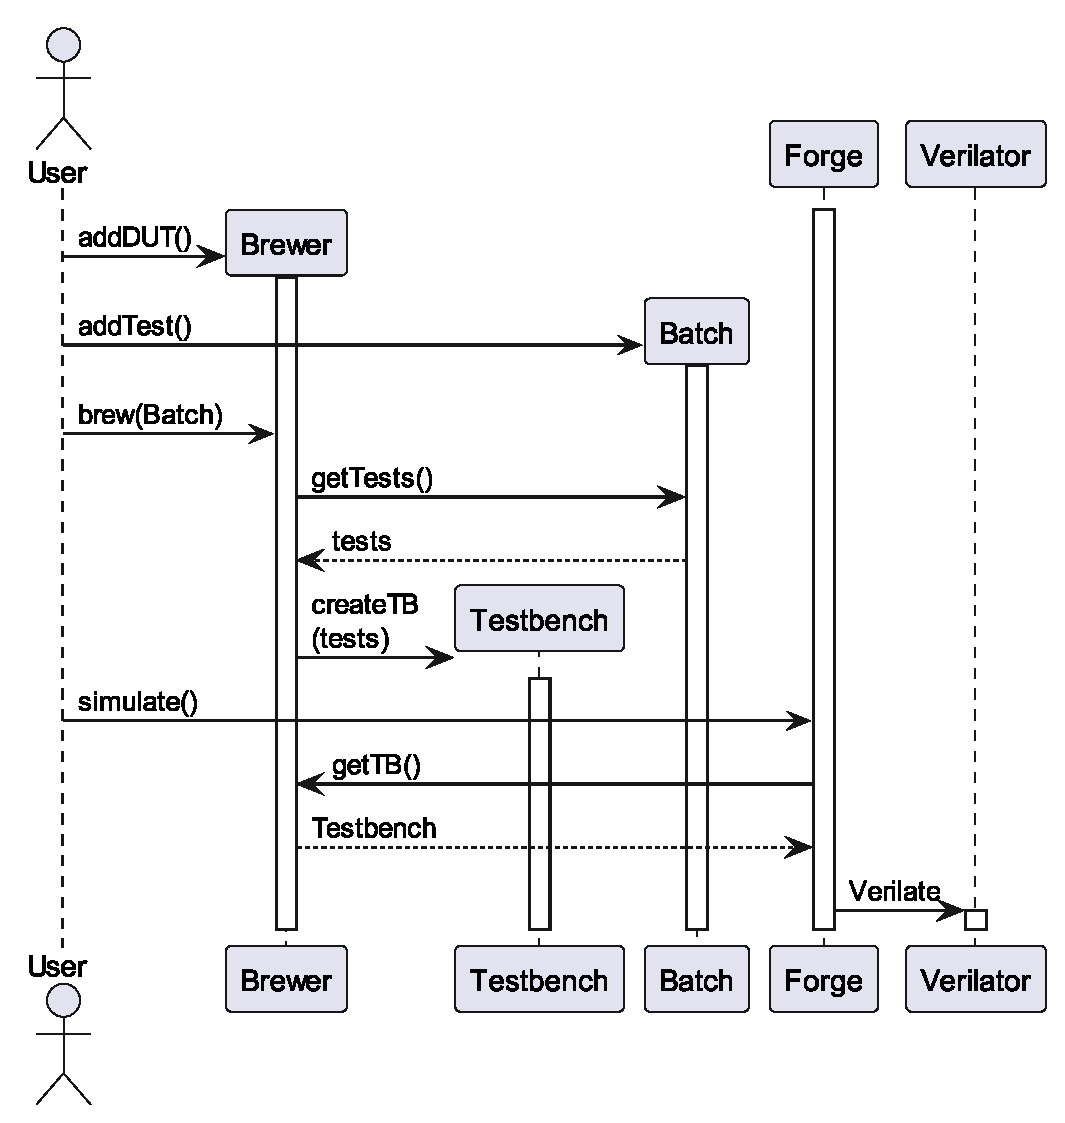
\includegraphics[width=.5\textwidth]{out/plantuml/seq/sequenceDiag.eps}
\end{figure}
The class diagram is shown on \cref{fig:classDiag}.
\begin{figure}
    \centering
    \caption{Class diagram showing the structure of SteelBrew}\label{fig:classDiag}
    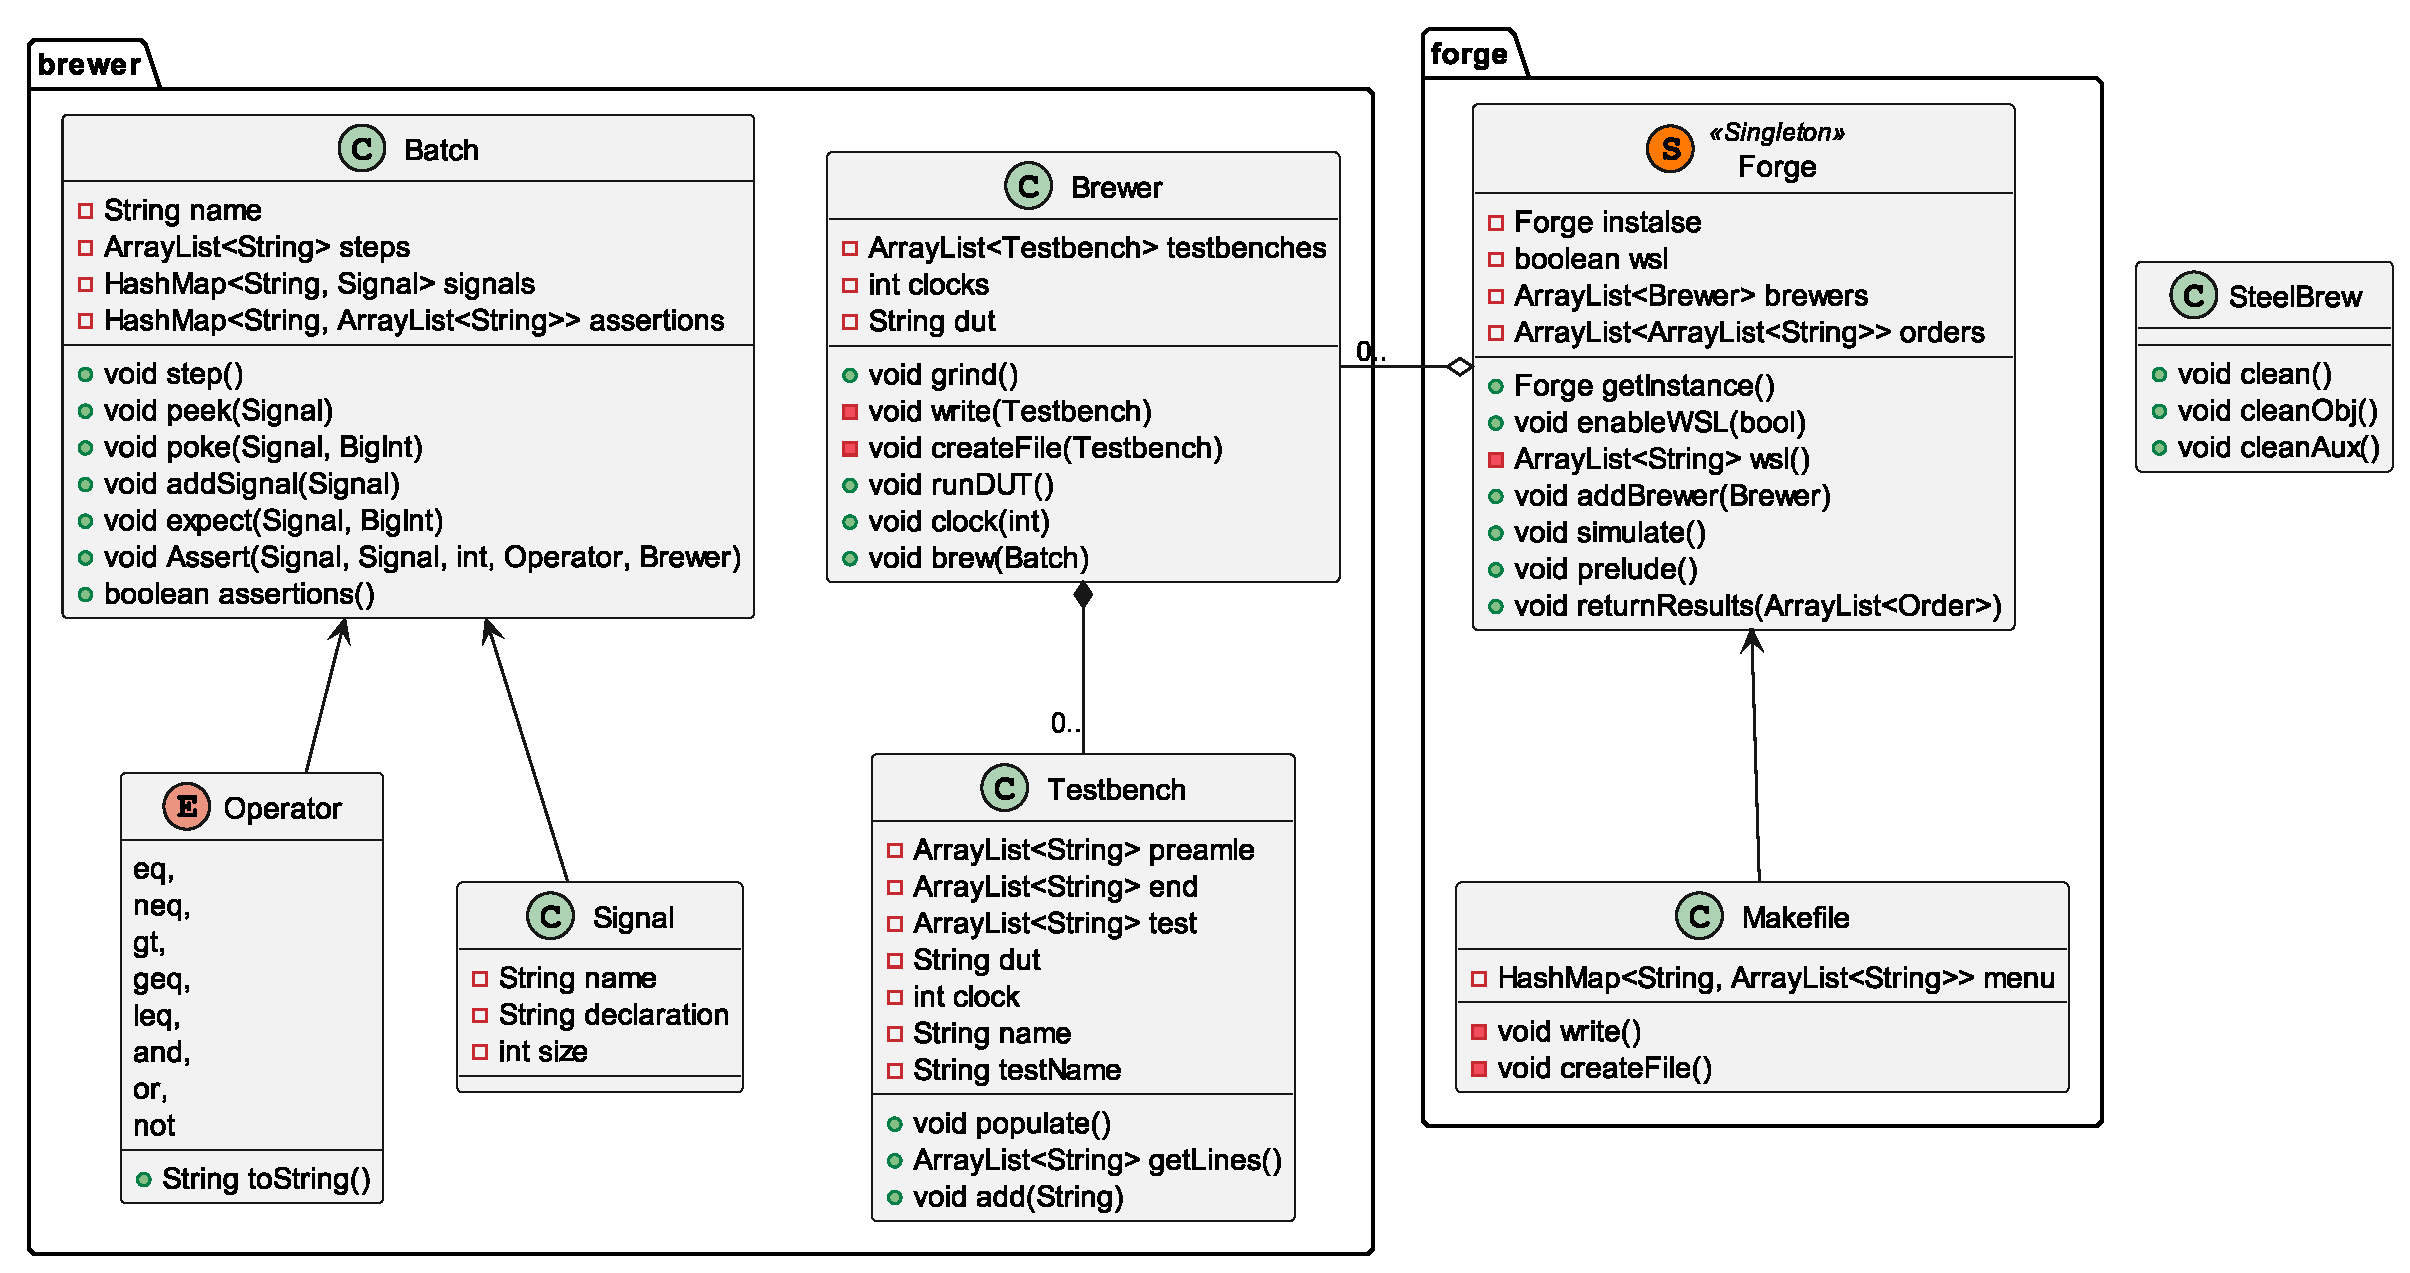
\includegraphics[width=\textwidth]{out/plantuml/classDiag/classDiag.eps}
\end{figure}
Notice that the Forge is a singleton. This was chosen to make access to the Forge easier and most importantly ensure that only one Forge is instantiated. The Forge handles the executed threads, and multiple instances could lead to race conditions. The Barista class has been omitted from the diagram but will be discussed further in \cref{sec:05}.
% LTeX: language=en-GB
% !TeX root = ..\Thesis.tex
\section{Implementation}\label{sec:06}
In this section the practical implementation is showcased and discussed. Each class is briefly summarised, and interesting solutions are shown.
\subsection{Build environment}
The project exists in a Gradle\footnote{Gradle on the web: \href{https://gradle.org/}{gradle.org}} build environment consisting of an app and a library. The reasoning is simple: This project is developed as a library that the developer can import into their own Java code. The app is a merely a demo of how the library can be used, while the library itself is the project. If the project should be published Gradle will easily publish it to the Maven central repo. The demo app is in the \texttt{app} folder and the project is in the \texttt{steelbrew} folder. The root folder contains two ALUs written in SystemVerilog to experiment on.
\subsection{SteelBrew}
This class is the entry point for the project. It has two purposes. First it instantiates the Forge as a singleton. Second it has auxiliary functions for cleaning files produced during simulation.
\subsection{Brewer}
The brewer class is constructed for each DUT to be tested. Upon construction, it adds itself to the Forge.\newline
When the user is ready to simulate the Forge calls the \mintinline{java}|void grind()| method that creates and fills out testbench files. The \mintinline{java}|void brew(Batch batch)| method shows how a batch of tests is used to create a testbench. The method is shown on \cref{lst:brew}.
\begin{listing}
    \centering
    \caption{Brewers brew method for creating a testbench from a batch of tests}\label{lst:brew}
    \begin{minted}{java}
        public void brew(Batch batch) {
        Testbench testbench = new Testbench(dut, batch.getName(), clocks);
        if (batch.assertions()) {
            HashMap<String, ArrayList<String>> assertions = batch.getAssertions();
            Set<String> functions = assertions.keySet();
            functions.forEach(f -> assertions.get(f).forEach(s -> testbench.add(s)));
            testbench.add("    while (sim_time < MAX_SIM_TIME) {\n");
            testbench.add("        dut->clk ^= 1;\n");
            testbench.add("        dut->eval();\n");
            testbench.add("        if(dut->clk == 1){\n");
            testbench.add("            posedge_cnt++;\n");
            testbench.add("        }\n");
            functions.forEach(f -> testbench.add(f+"\n"));
            testbench.add("        m_trace->dump(sim_time);\n");
            testbench.add("        sim_time++;\n");
            testbench.add("    }\n");
            testbench.add("\n");
        }
        ArrayList<String> steps = batch.getSteps();
        for (String step : steps) {
            testbench.add(step);
        }
        testbenches.add(testbench);
    }
    \end{minted}
\end{listing}
\cref{lst:brew} illustrates how tests are converted into testbench functions.
\subsection{Testbench}
\begin{listing}
    \centering
    \caption{Example of inserting custom names into the testbench}\label{lst:tb}
    \begin{minted}{java}
        preamble.add("int main(int argc, char** argv, char** env) {\n");
        preamble.add("    V" + testName + " *dut = new V" + testName + ";\n");
    \end{minted}
\end{listing}
The Testbench class holds all the necessary lines to make a testbench work. The \mintinline{java}|void add(String string)| method can then be used to add test lines to the testbench. The Brewer then assembles the file. \cref{lst:tb} shows how the testbench names are assigned. When a testbench is created the variable \texttt{testName} combines the name of the DUT, with the name of the test.
\subsection{Batch}
The Batch class defines the test methods \mintinline{java}|step()|, \mintinline{java}|peek()|, \mintinline{java}|poke()|, \mintinline{java}|expect()| and \mintinline{java}|Assert()|. The peek method is interesting here, as it writes to stdout with its result. This can be seen on \cref{lst:peek}.
\begin{listing}
    \centering
    \caption{The peek method}\label{lst:peek}
    \begin{minted}[breaklines]{java}
    public void peek(Signal signal) {
        steps.add("std::cout << \"\\n Peek on " + signal.getName() + ": \" << (int)(dut->" + signal.getName()
                + ") << \" @ simtime: \" << sim_time << std::endl;\n");
    }
    \end{minted}
\end{listing}
The assert method is also of interest. It takes two signals and an operator and then constructs a C++ method, that looks for some comparison, depending on the chosen operator. In \cref{lst:brew} the assertions are put into a testbench. The values of the assertion HashMap contains the method definition. The key is the function call. In \cref{lst:brew} the methods are defined early in the testbench and the call is the placed in a loop that evaluates every clock cycle, thus the assertion has to hold throughout the DUT evaluation. The two helper classes Operator and Signal will briefly be explained.
\subsubsection{Operator}
The operator is a Java enum that comprises all the operators for comparison. The enum has a \mintinline{java}|toString()| method. If an assertion is added as such,\newline\mintinline{java}|batch.Assert(signal, signal2, 1, Operator.neq, alu);| the assert method uses the toString method to convert \texttt{neq} to ``\(!=\)'' when inserted in the C++ method.
\subsubsection{Signal}
The Signal class is a POJO\footnote{\textbf{P}lain \textbf{O}ld \textbf{J}ava \textbf{O}bject} that defines the signal with a name, signal size and declaration, when used as a variable in C++.
\subsection{Makefile}
The Makefile class is used to create a GNU Make Makefile to simplify process calls from the Forger. This can be seen on \cref{lst:make}.
\begin{listing}
    \centering
    \caption{The write method that creates the recipes for the verilation, compilation and execution of simulations}\label{lst:make}
    \begin{minted}[breaklines]{java}
    private void write() {
        try {
            FileWriter writer = new FileWriter("Makefile");
            Set<String> duts = menu.keySet();
            for (String dut : duts) {
                ArrayList<String> tests = menu.get(dut);
                for (String test : tests) {
                    writer.write(".PHONY: " + test + "\n");
                    writer.write("\n");
                    writer.write(test + ": waveform" + test + ".vcd\n");
                    writer.write("\n");
                }
                for (String test : tests) {
                    writer.write("waveform" + test + ".vcd: ./obj_dir/V" + test + "\n");
                    writer.write("\t@./obj_dir/V" + test + "\n");
                    writer.write("\n");
                    writer.write("./obj_dir/V" + test + ": .stamp." + test + ".verilate\n");
                    writer.write("\t@echo \"### Building executable ###\"\n");
                    writer.write("\tmake -C obj_dir -f V" + test + ".mk V" + test + "\n");
                    writer.write("\n");
                    writer.write(".stamp." + test + ".verilate: " + dut + ".sv " + "tb_" + test + ".cpp\n");
                    writer.write("\t@echo \"### VERILATING ###\"\n");
                    writer.write("\tverilator --trace -cc " + dut + ".sv --exe tb_" + test + ".cpp --prefix V"
                            + test + "\n");
                    writer.write("\t@touch .stamp." + test + ".verilate\n");
                    writer.write("\n");
                }
            }
            writer.write(".PHONY: clean\n");
            writer.write("clean:\n");
            writer.write("\trm -rf .stamp.*;\n");
            writer.write("\trm -rf ./obj_dir\n");
            writer.write("\trm -rf *.vcd\n");
            writer.close();
        } catch (IOException e) {
            e.printStackTrace();
        }
    }
    \end{minted}
\end{listing}
Lines 8-11 gives the test recipe a name, and calls for a waveform creation. 14-26 then recursively goes through the recipes:
\begin{enumerate}
    \item The waveform depends on the executable.
    \item The executable depends on the verilation stamp (an empty file telling Make that verilation is not necessary on repeated makes).
    \item The stamp then depends on verilating the testbench and DUT.
\end{enumerate}
\subsection{Forge}
The Forge is where processes are handled. It is instantiated as a singleton, which means it is always accessible, and only one copy exists, making race-conditions less likely. The constructor also allows for lazy initialisation, meaning it is initialised when the \mintinline{java}|Forge.getInstance()| method is first called.\newline
Forge has a \mintinline{java}|wsl()| method that solves the problem that Verilator does not ship binaries for Windows. However, if Windows Subsystem for Linux is installed with Verilator, Verilator can be called from a Windows terminal with the command \mintinline{bash}|wsl -d Ubuntu <Command>|.
The Forge executes simulations by calling \mintinline{java}|prelude()| which prompts the brewers to create testbench files. Afterwards the method creates an instance of Makefile and collects a list of all tests to be executed. The lists contain the command call for the process to start. Forge then constructs an instance of the Barista class, which in turn deals with a multithreaded approach.
\subsubsection{Barista}
The Barista class is a helper class for the Forge class, that creates string builders that in turn executes the ``make'' command and saves stdout and stderr. Barista runs a test on its own thread, enabling concurrent simulation. Upon completion Barista calls \mintinline{java}|Forge.returnResults()|, which then prints the output of the tests, thus completing the simulations.
% LTeX: language=en-GB
% !TeX root = ..\Thesis.tex
\section{The final product}\label{sec:07}
This section will demonstrate the resulting workflow of the project for some various setups.
\subsection{Running the device}
The simplest workflow is running a DUT for some number of cycles. Consider \cref{lst:runDut}.
\begin{listing}
    \centering
    \caption{Running an ALU for 40 cycles}\label{lst:runDut}
    \begin{minted}{java}
        SteelBrew steelBrew = new SteelBrew();
        steelBrew.clean();
        Forge.enableWSL(true);
        Brewer alu = new Brewer("alu");
        alu.clocks(40);
        alu.runDUT();
        Forge.simulate();
    \end{minted}
\end{listing}
Line 1 initialises SteelBrew and the Forge. Hereafter the root folder is cleaned for leftover files from previous simulations. Line 3 enables the Windows Subsystem for Linux support. On line 4 the ALU is added as the DUT. Line 5 sets the number of running cycles to 40 and 6 creates a testbench that simply runs the DUT for 40 cycles. On line 7 the program begins the simulation. The resulting file \texttt{waveformalurun.vcd} can then be inspected. The resulting screenshot is shown on \cref{fig:runDut}.
\begin{figure}
    \centering
    \caption{Waveform after running the ALU for 40 cycles}\label{fig:runDut}
    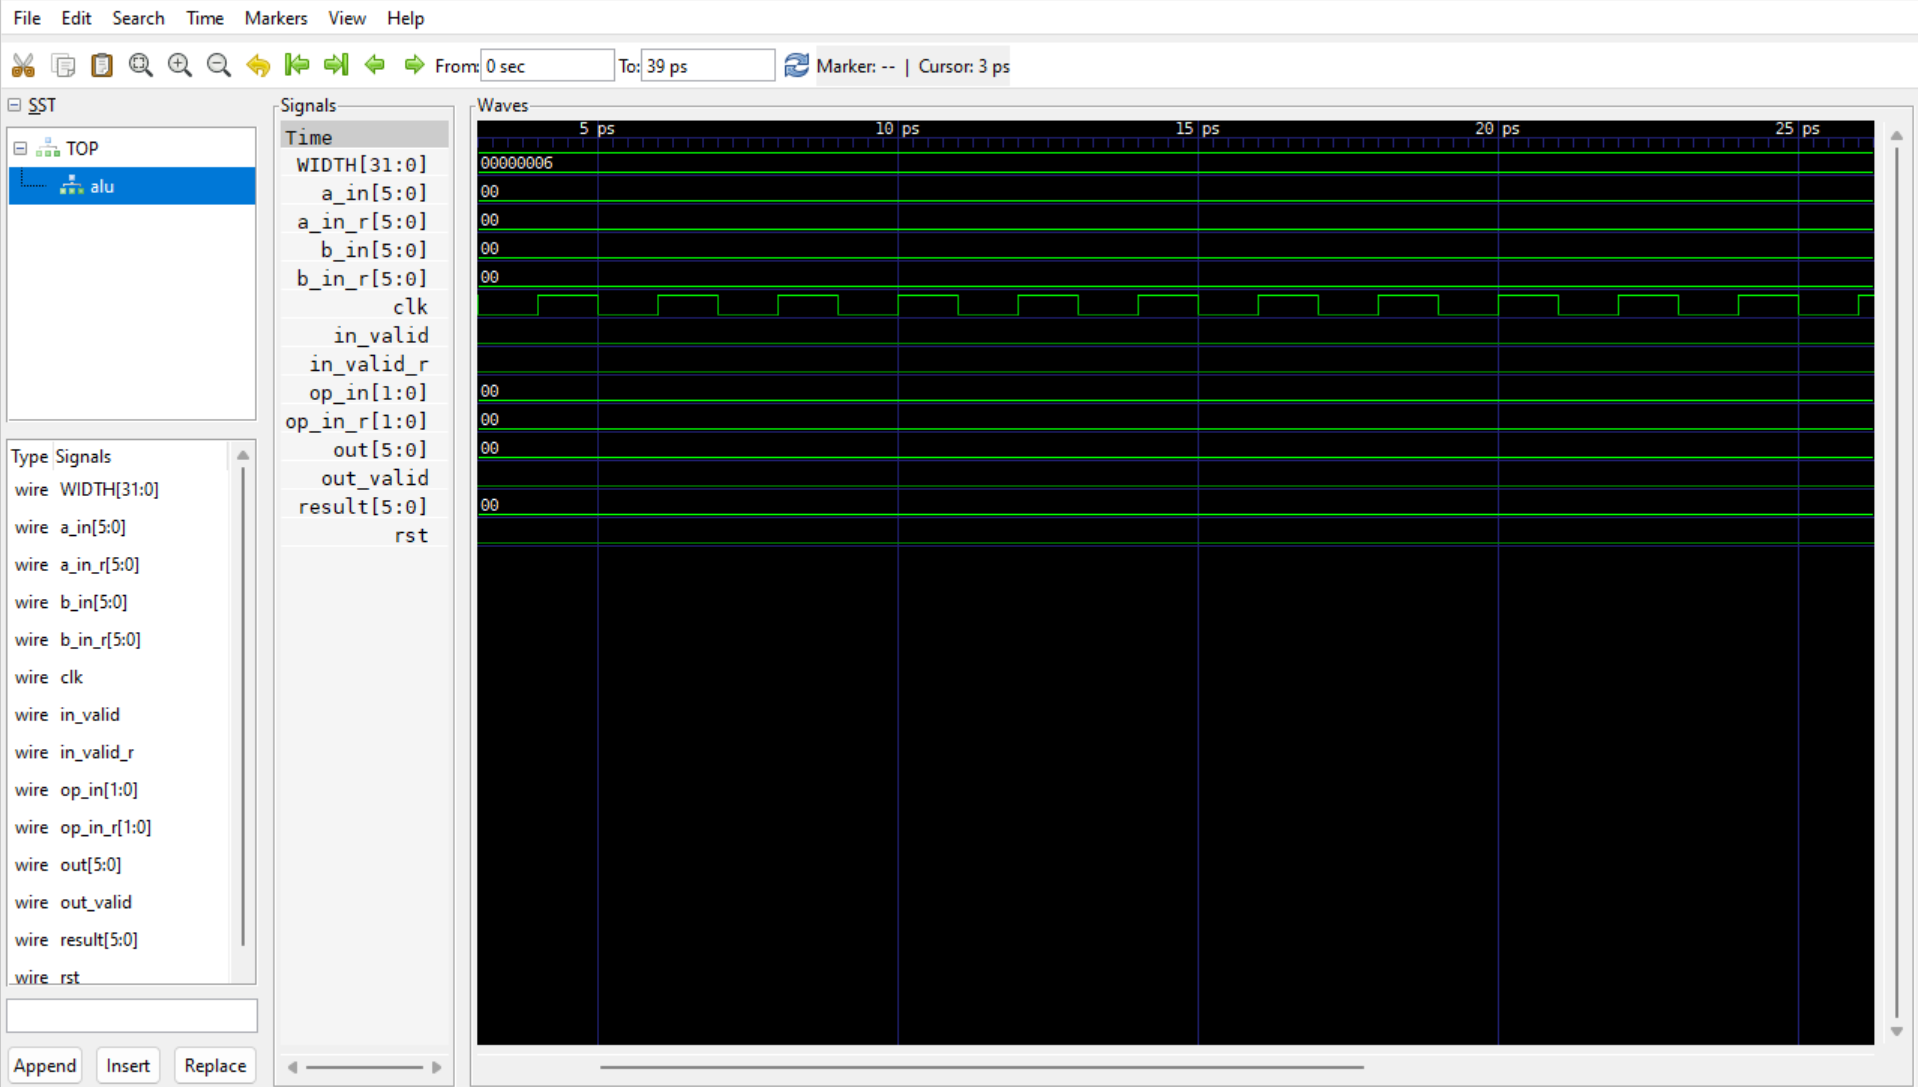
\includegraphics[width=.8\textwidth]{graphics/runDUT.png}
\end{figure}
As seen from the figure, the ALU ran from 0 to 39 ps and the \texttt{clk} signal is behaving as expected. The simplest case works.
\subsection{Peek, poke and step}
For the next workflow, the listing is shown on \cref{lst:peekpokestep}.
\begin{listing}
    \centering
    \caption{Peek, poke, and step used on an ALU}\label{lst:peekpokestep}
    \begin{minted}{java}
        SteelBrew steelBrew = new SteelBrew();
        steelBrew.clean();
        Forge.enableWSL(true);
        Brewer alu = new Brewer("alu");
        Batch batch = new Batch("PeekPokeStep");
        Signal signal = new Signal("in_valid", 1);
        batch.addSignal(signal);
        batch.peek(signal);
        batch.poke(signal, BigInteger.ONE);
        batch.step();
        batch.peek(signal);
        batch.step();
        batch.poke(signal, BigInteger.ZERO);
        batch.step();
        batch.peek(signal);
        batch.step();
        batch.step();
        alu.brew(batch);
        Forge.simulate();
    \end{minted}
\end{listing}
Lines 1-5 is seen in the previous example. On line 6 the variable \texttt{signal} is pointed to ``\texttt{in\_valid}'', and on line 7 the signal is added to the batch. Lines 8–15 peeks at the signal, changes it to 1, peeks and changes it to 0, with some clock steps in-between. 16-17 starts the simulation. \cref{fig:peekpokestep} shows the resulting console output and \cref{fig:peekpokestepWave} shows the signal.
\begin{figure}
    \centering
    \caption{Console output after using peek, poke and step on the ALU}\label{fig:peekpokestep}
    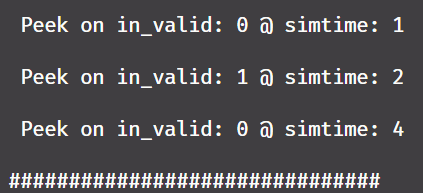
\includegraphics[width=.3\textwidth]{graphics/peekpokestep.png}
\end{figure}
\begin{figure}
    \centering
    \caption{Waveform changes with and poke}\label{fig:peekpokestepWave}
    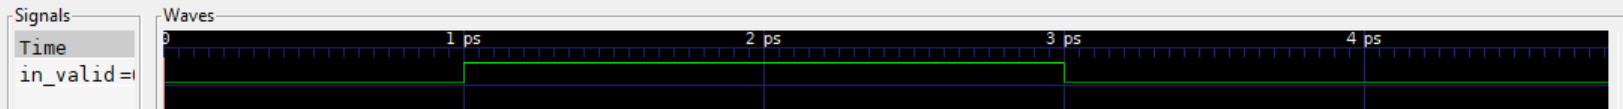
\includegraphics[width=\textwidth]{graphics/peekpokestepWave.png}
\end{figure}
The wave and the console output behaves as expected.
\subsection{Expect}
This next workflow demonstrate how to look for expected values. Consider \cref{lst:expect}.
\begin{listing}
    \centering
    \caption{Expecting signal in the ALU}\label{lst:expect}
    \begin{minted}{java}
        SteelBrew steelBrew = new SteelBrew();
        steelBrew.clean();
        Forge.enableWSL(true);
        Brewer alu = new Brewer("alu");
        Batch batch = new Batch("Expect");
        Signal signal = new Signal("in_valid", 1);
        batch.addSignal(signal);
        batch.step();
        batch.expect(signal, BigInteger.ONE);
        batch.peek(signal);
        batch.step();
        alu.brew(batch);
        Forge.simulate();
    \end{minted}
\end{listing}
The new addition here is line 9. We expect the signal to be a 1. \cref{fig:expectConsole} shows the console output.
\begin{figure}
    \centering
    \caption{Console output after using expect on the ALU}\label{fig:expectConsole}
    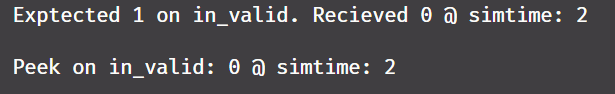
\includegraphics[width=.5\textwidth]{graphics/expectConsole.png}
\end{figure}
Exactly as expected.
\subsection{Assertions}
Regrettably, the assertion methods did not work as expected. After rigorous experimentation, it would seem like the approach employed in the Assert method is inherently flawed. Placing the while loop in the testbench is needed for the current assertion-logic, however it rules out the possibility for peek and poke during a batch containing assertions. Further investigation is needed. Perhaps some randomised initial conditions combined with the expect method, would stand in for assertions, but this is truly not the way either.
\subsection{Concurrency}
When executing multiple batches, the forge successfully runs multiple threads as seen on \cref{fig:concurr}.
\begin{figure}
    \centering
    \caption{Multiple instances of Verilator created by Barista}\label{fig:concurr}
    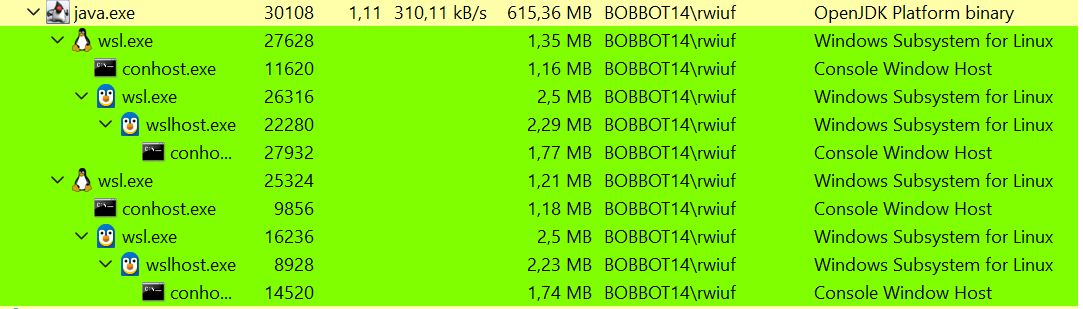
\includegraphics[width=.8\textwidth]{graphics/concurrency.png}
\end{figure}
This combined with Verilator's lightweight approach, and possibly, by employing its multithreading capabilities could dramatically speed up the verification process.
\subsection{Further development}
The groundwork is laid for further development. The development tasks would be as follows:
\begin{enumerate}
    \item Implement working Assertions.
    \item Employ Verilator multithreading.
    \item Expand assertions with assume and cover logic.
\end{enumerate}
The project as-is would be easily extendable with other testing capabilities, and as it is written in Java, the user could use their own logic, to prepare and execute tests.
% LTeX: language=en-GB
% !TeX root = ..\Thesis.tex
\section{Conclusion}\label{sec:08}
The project did not reach its final goal: Implementing Assertion Based Verification.\newline
However, other goals were reached. SteelBrew communicates with Verilator and using the Makefile, rather efficiently. The basic manipulation methods works as expected making the project employable as of this moment. The project further translates the tests in a way that makes parallel execution doable. The concurrency works as expected, and if more tests are added to the batches, this is a tool that can verify multiple DUTs in multiple setups simultaneously.
%Bibliography herunder:
\newpage
\printbibliography[heading=bibintoc]
\listoffigures
\listoftables
\lstlistoflistings
%\newpage

%Appendicer herunder:

%\input{Appendix.tex}

\end{document}
